\documentclass[tikz]{standalone}

\pagestyle{empty}


\usepackage{amsmath}
\usepackage{tikz}
\usepackage{graphicx}
\usetikzlibrary{positioning,calc,fit,decorations.pathreplacing,arrows,positioning,backgrounds}

% Font settings:
\renewcommand{\familydefault}{\sfdefault}
\usepackage{pxfonts}
\newcommand{\figf}{\sffamily\bfseries\small} %Defines the font used for the labelling of figure panels.


% Color settings:
%\definecolor{hivc}{cmyk}{0,0.80,0.83,0.13}                %\definecolor{hivc}{HTML}{DE2D26}
\definecolor{hivc}{RGB}{24,116,205}
\definecolor{selfc}{cmyk}{0,0,0,0.6}                      %\colorlet{selfc}{gray!80!white}
\definecolor{Rblue}{RGB}{100,149,237}


\begin{document}
\scriptsize

\begin{tikzpicture}[anchor=north west]

    \begin{scope}
      \begin{scope}[xshift=1cm, yshift=-3.5cm]
      \draw[fill=gray!50!white] (0,0) rectangle +(1,1);
      \node[anchor=center] at (0.5, 0.5) {+};
      \draw (0,1) rectangle +(1,1);
      \node[anchor=center] at (0.5, 1.5) {-};
      \draw[fill=gray!50!white] (1,0) rectangle +(1,1);
      \node[anchor=center] at (1.5, 0.5) {+};
      \draw[fill=gray!50!white] (1,1) rectangle +(1,1);
      \node[anchor=center] at (1.5, 1.5) {+};
      \draw (2,0) rectangle +(1,1);
      \node[anchor=center] at (2.5, 0.5) {-};
      \draw[fill=gray!50!white] (2,1) rectangle +(1,1);
      \node[anchor=center] at (2.5, 1.5) {+};
      
      \node[anchor = east] at (0,0.5) {stop};
      \node[anchor = east] at (0,1.5) {go};
      \node[anchor = south] at (0.5, 2) {NM};
      \node[anchor = south] at (1.5, 2) {I-RW};
      \node[anchor = south] at (2.5, 2) {P-RW};
      \end{scope}
      \node at (0,0) {\figf A};
    \end{scope}
    
    \begin{scope}[xshift=5cm]
      \node at (0,0) {\includegraphics[page=5, scale=0.7]{../barrier.pdf}};
      \node at (0,0) {\figf B};
    \end{scope}

\end{tikzpicture}

\newpage
\begin{tikzpicture}[anchor=north west]
	
	\clip (0,0) rectangle +(15.5,-9.85);

	 \begin{scope}
      \node at (0.2,-0.5) {\includegraphics{../plots/energies.pdf}};
      \node at (0,0) {\figf A};
      \node[anchor = center] at (4.5,-0.4) {$\lambda_\text{act}$ = 80};
      \node[anchor = center] at (12,-0.4) {$\lambda_\text{act}$ = 160};
    \end{scope}
    
    
    \begin{scope}[yshift=-6.7cm]
    
		\begin{scope}
		  \begin{scope}[yshift=-0.5cm]
			\begin{scope}
			  \clip (0.8,0) rectangle +(2.7,-2.5);
			  \foreach \x in {0,...,19}
			  {\pgfmathtruncatemacro{\t}{\x+436}
				\node at (0,-0.1*\x) {\includegraphics[width=0.5\textwidth]{../output/stopgo-t\t.png}};}
			\end{scope}
			\draw[->] (0.7,-0.1) -- (0.7,-2.1);
			\node[anchor=center,rotate=90] at (0.4,-1.1) {\sffamily\footnotesize time (MCS)};
		  \end{scope}
	  
		  \node at (0,0) {\figf B};
		\end{scope}
  
		\begin{scope}[xshift=3.8cm]
		  \node at (0,-0.2) {\includegraphics{../plots/diagram.pdf}};
		  \node at (0,0) {\figf C};
		  \node[anchor = center] at (2.65,-0.4) {$\lambda_\text{act}$ = 80};
      	  \node[anchor = center] at (5.52,-0.4) {$\lambda_\text{act}$ = 160};
		\end{scope}

		\begin{scope}[xshift=10.5cm]
		  \node at (0,-0.2) {\includegraphics{../plots/lambda-energy.pdf}};
		  \node at (0,0) {\figf D};
		\end{scope}
	\end{scope}

\end{tikzpicture}



\end{document}